Cuts must be applied to data to give a set of ``good electrons''. Cuts are a defined set of conditions that must be met by an event to be classified as ``good''. A good event is one in which the detected particle is an electron that deep inelastically scattered from the target. In this analysis, the cuts can be classified in two categories: Particle Identification and Acceptance. Particle Identification cuts are used to ensure that all events being studied are electrons. Acceptance cuts are used to ensure that all events passed through areas of the spectrometer that are well constrained by the spectrometer optics.

\subsection{Particle Identification}

Particle Identification (PID) cuts are applied to the detectors in the HRSs. The first PID cut is referred to as the ``Trigger 2'' cut. This cut requires that an event fires Trigger 2 (Trigger 5 for the RHRS) which is the (S0 \&\& S2) \&\& Cherenkov trigger. This cut requires that S0 and S2 fire, which will ensure proper event timing and tracking. Ensuring that the Cherenkov fires is the first step to limiting the events to electrons. As described in Section \ref{sec:cer}, the Cherenkov will, in most cases, only fire for electrons due to the 4.8 GeV/\textit{c} momentum threshold for pion detection.

The next cut is the ``1-Track'' cut. This cut requires that an event must have only one track through the spectrometer associated with it. A single track assures that the event corresponds to a single electron. When multiple tracks are present, there is a risk that tracking and spectrometer readings will be incorrect.

There is a cut placed on the $W^2$ of an event. The goal of MARATHON is to measure the DIS cross section ratios. A cut on $W^2$ must be placed in order to ensure that all events are from the DIS region and to reject events that originate from Resonance scattering. This cut is placed for $W^2>3$  GeV$^2$/\textit{c}$^4$.

A cut is placed on the Cherenkov signal. This cut is placed on the ADC spectrum of the Cherenkov. For the LHRS the cut is at 1500; the cut is placed at 2000 for the RHRS. While the Cherenkov will generally only fire for electrons, there are a small number of high momentum pions that are capable of creating a signal. The high momentum threshold for pions means that any pions that do create a signal will create a very small signal. This can be seen in Figure \ref{fig:cer_pid}. By placing this cut, the pion peak is completely removed while the electron peak is nearly completely allowed to pass.

The final PID cut is on the ratio of the energy of the particle to the momentum of the track ($E/p$). For electrons, which have a low mass compared to the energy scale of the experiment, the $E/p$ is expected to be approximately 1. Any particle of larger mass that passes the ``Trigger 2'' cut (and thus created a Cherenkov signal) will have an $E/p$ value significantly smaller than 1. In order to eliminate these non-electron events a cut on $E/p$ is placed at $0.7$ for both arms. This spectrum can be seen in Figure \ref{fig:cal_pid}.

The Cherenkov and Calorimeter cuts are needed to work in tandem to completely remove non-electron events. This can be seen clearly by plotting the two spectra on a 2D histogram. As shown in Figure \ref{fig:cervcal_pid}, both cuts are needed to isolate the electron signals.

\begin{figure}
\begin{center}
	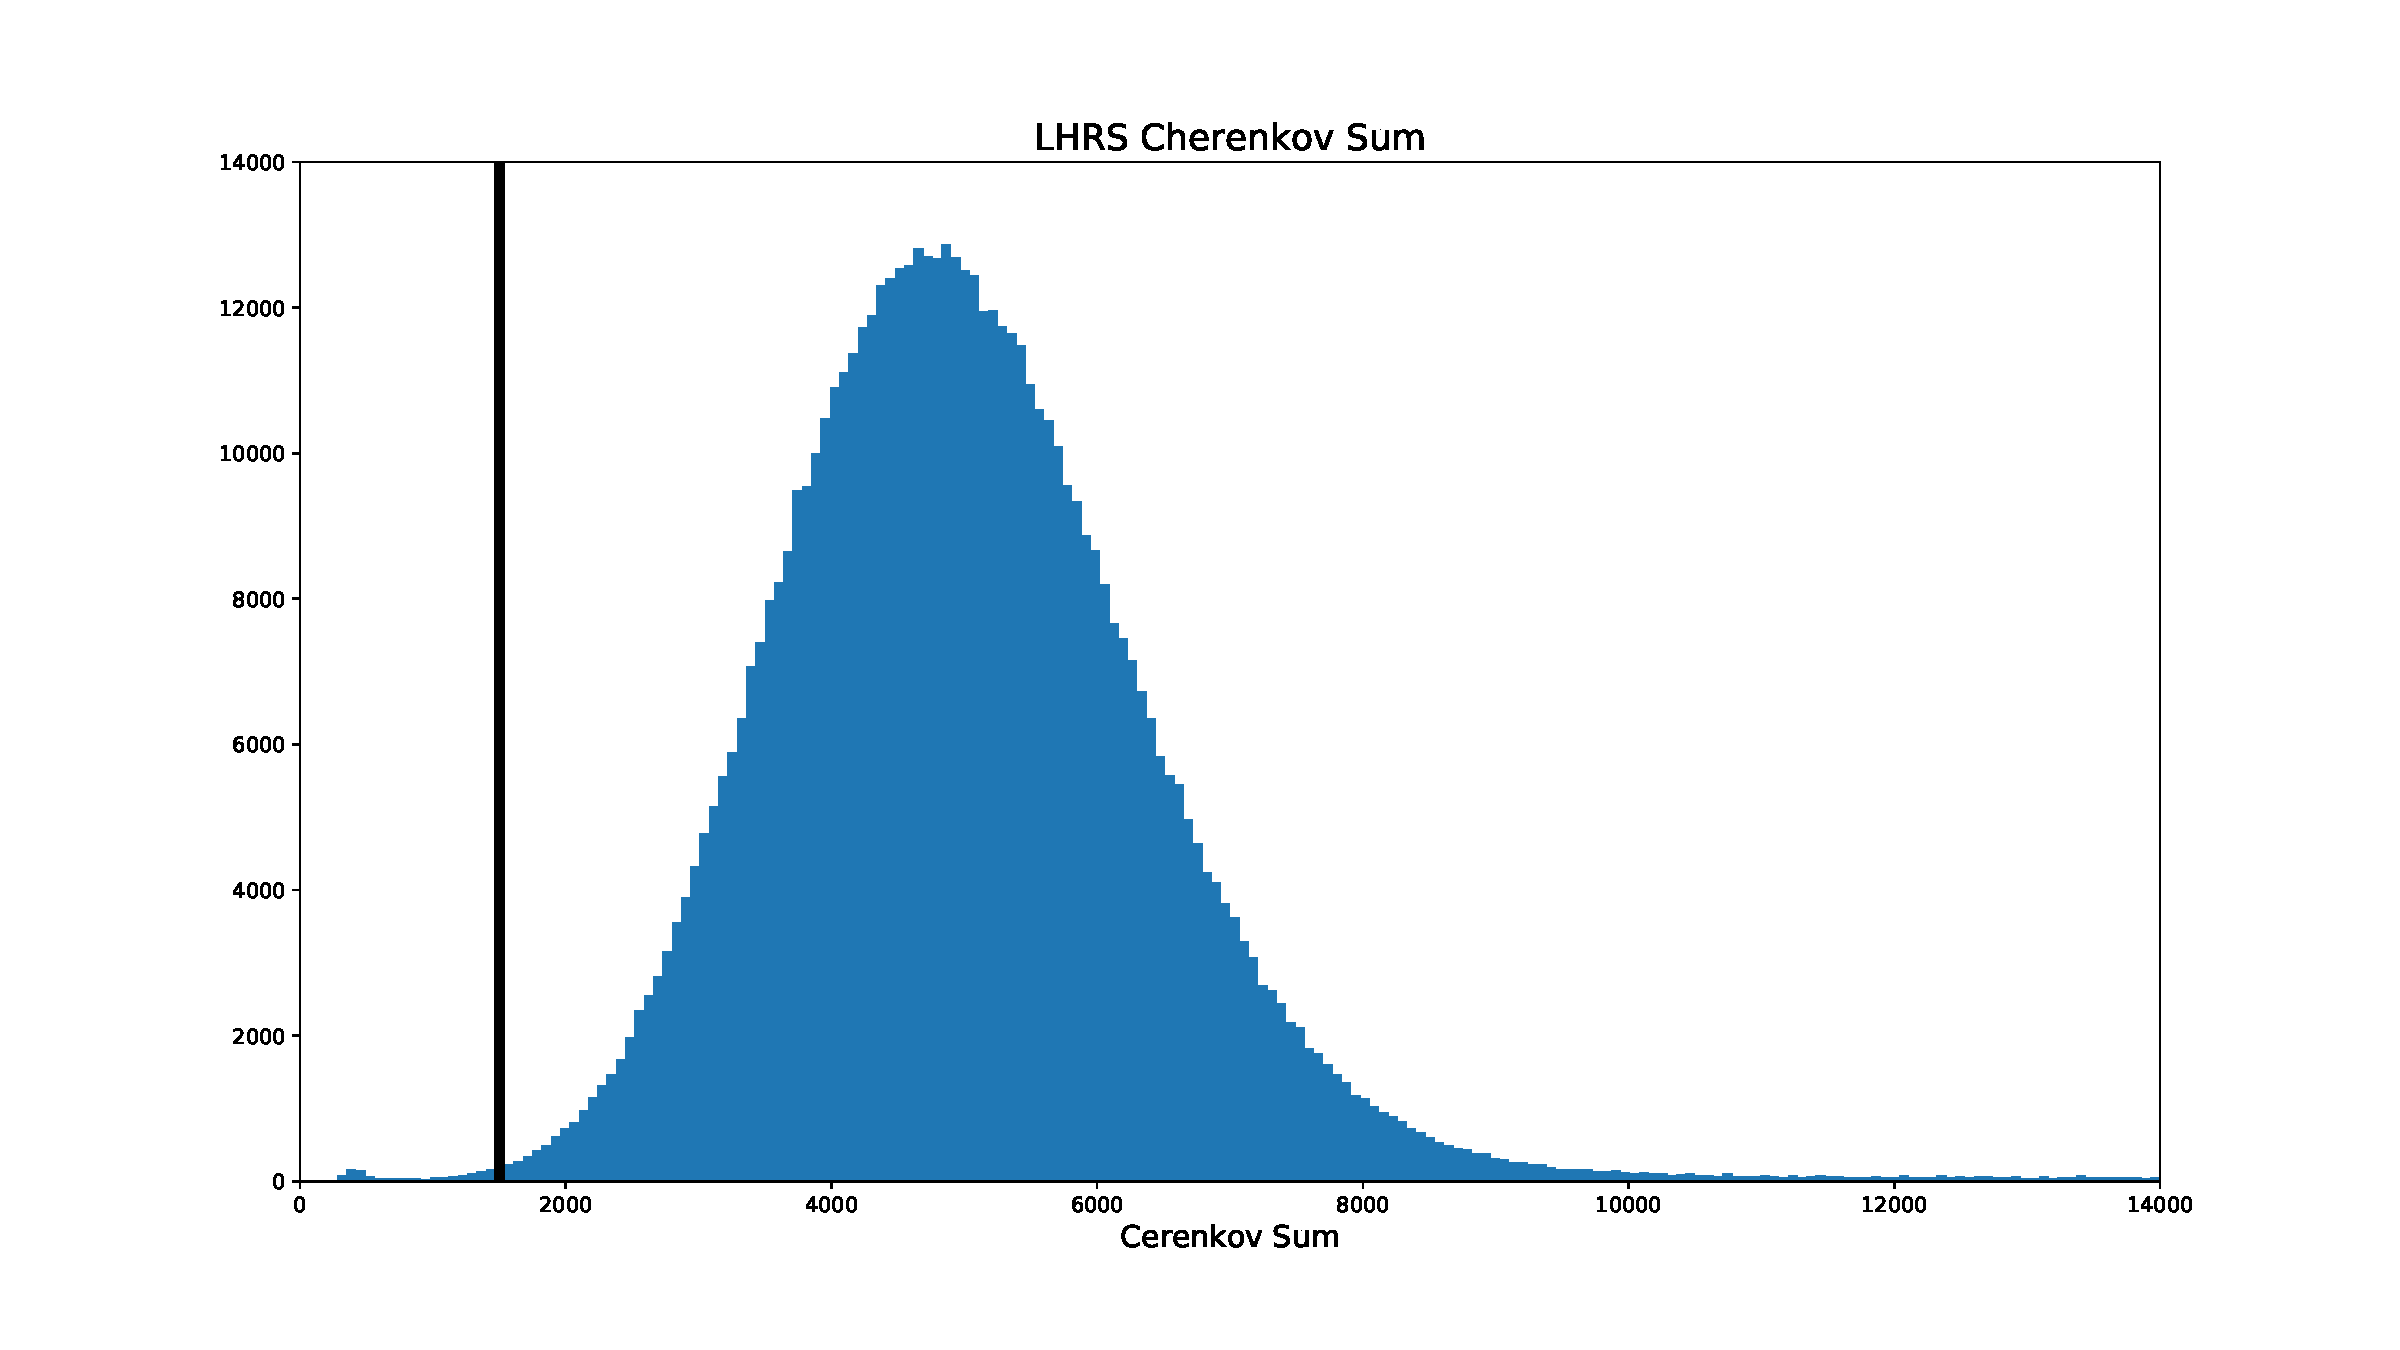
\includegraphics[width=\textwidth]{./analysis/fig/LCer_pid.pdf}
	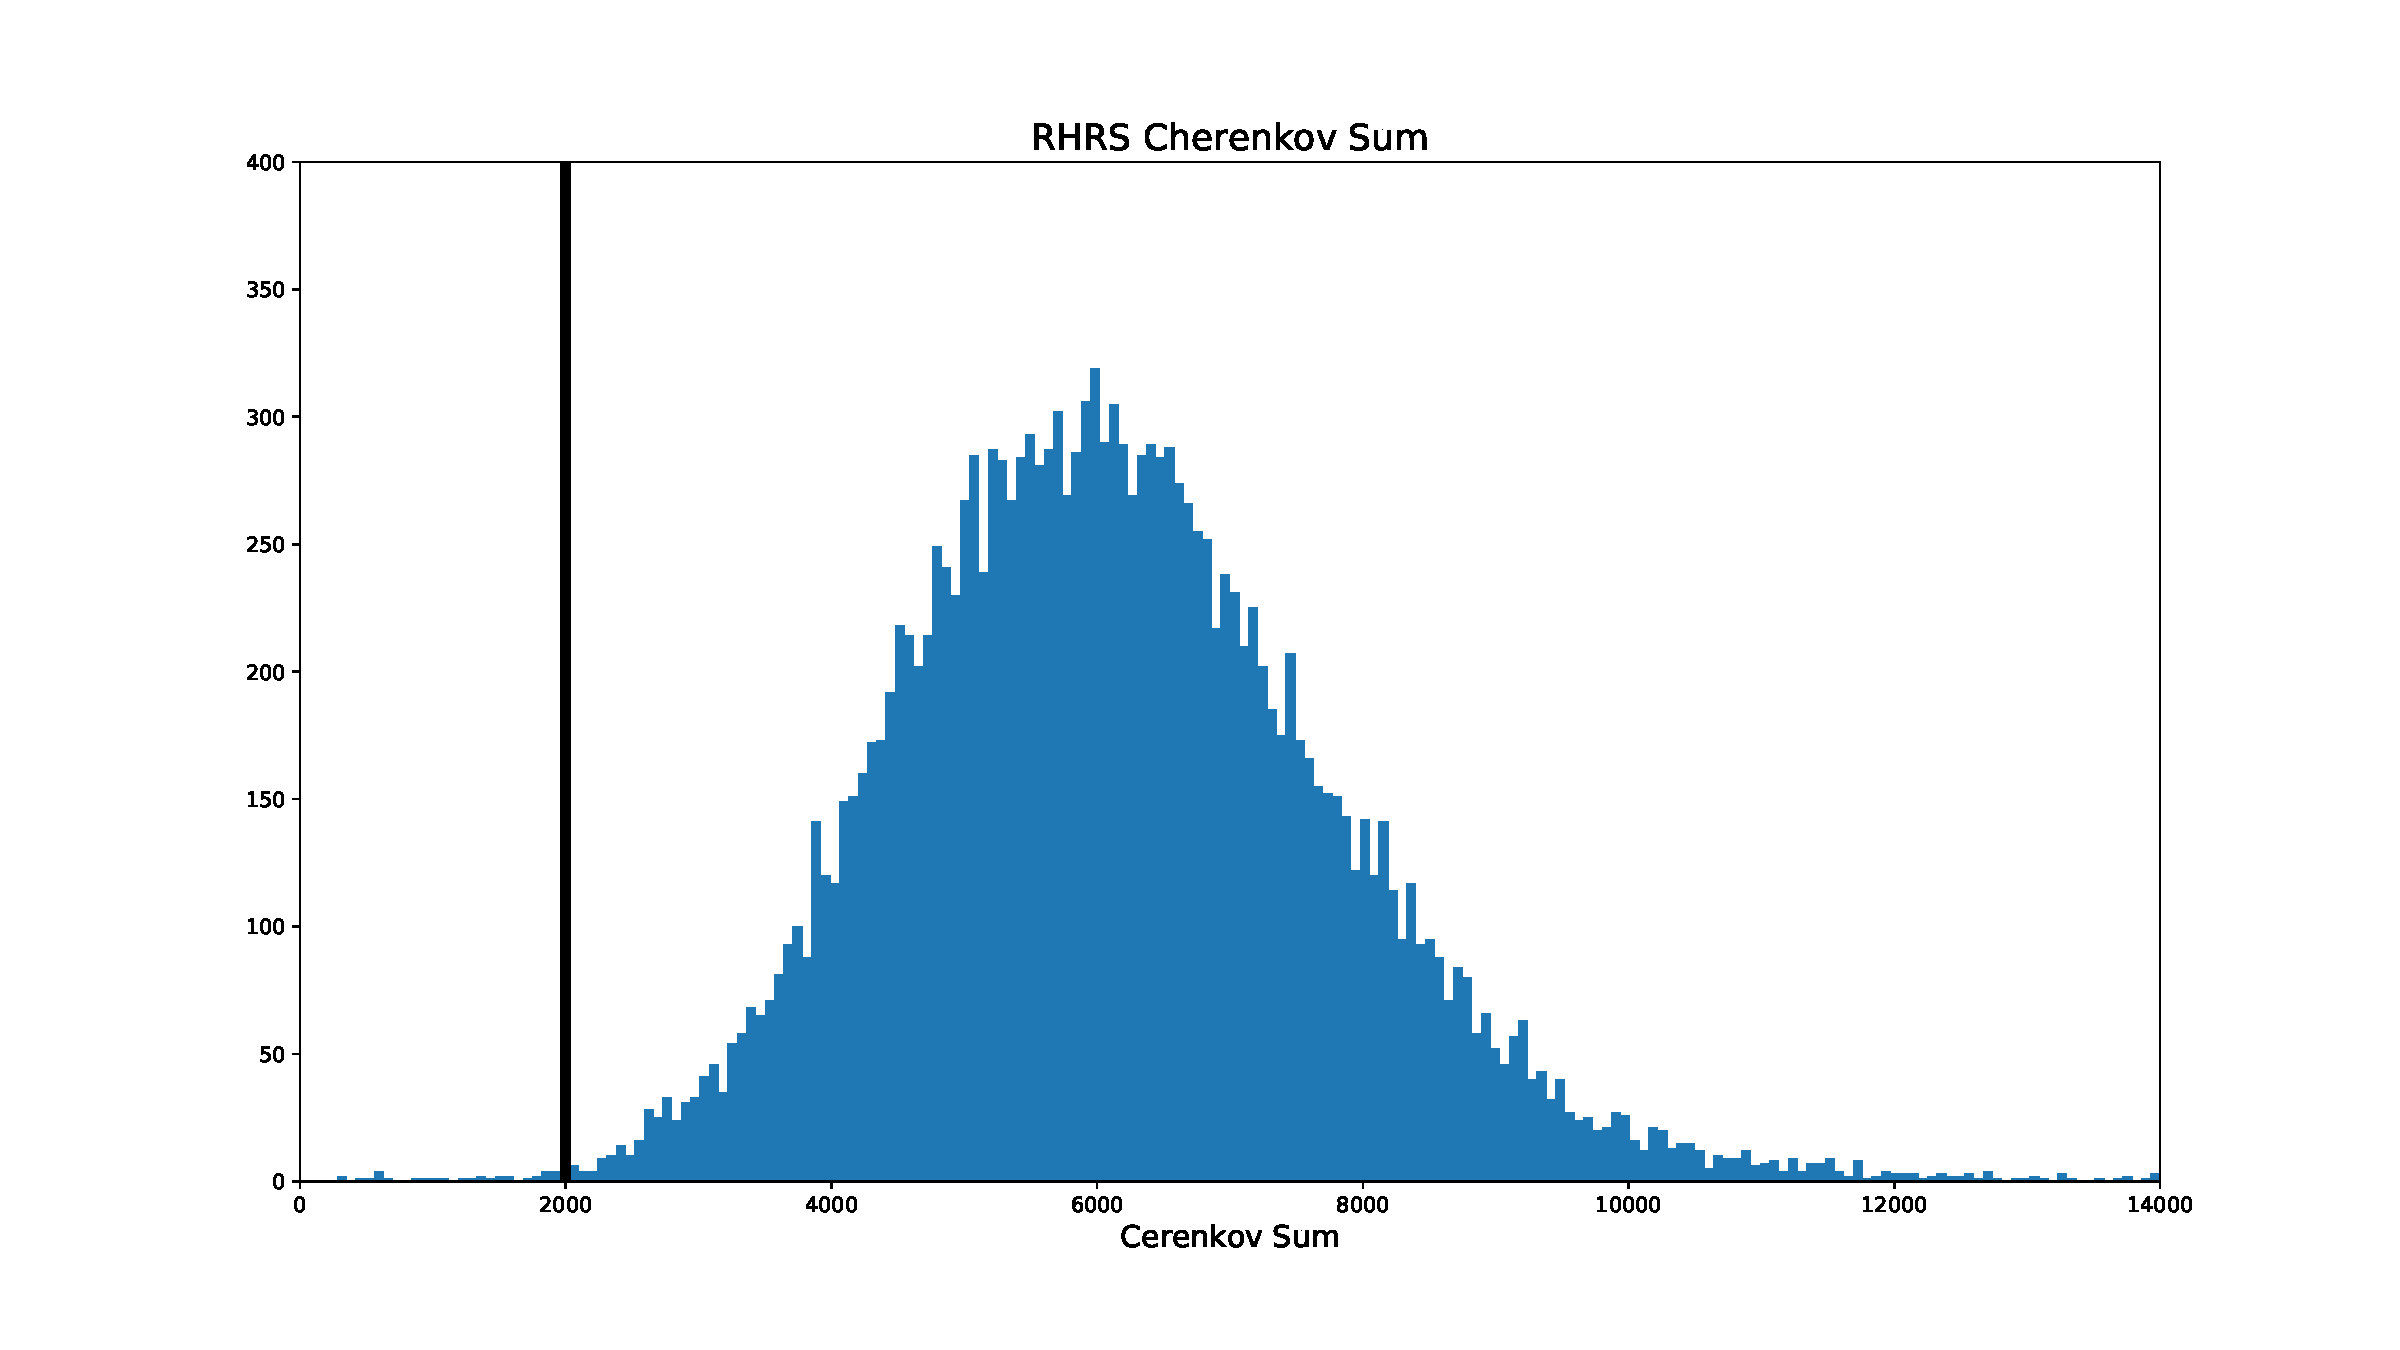
\includegraphics[width=\textwidth]{./analysis/fig/RCer_pid.pdf}
	\caption{These plots show the Cherenkov Sum for both the LHRS and RHRS. All cuts are applied except for the PID cut on the Cherenkov Sum. The LHRS plot shows events from kinematic 0 while the RHRS plot shows events from kinematic 16. The black lines show the where the cuts are applied.}
	\label{fig:cer_pid}
\end{center}
\end{figure}

\begin{figure}
\begin{center}
	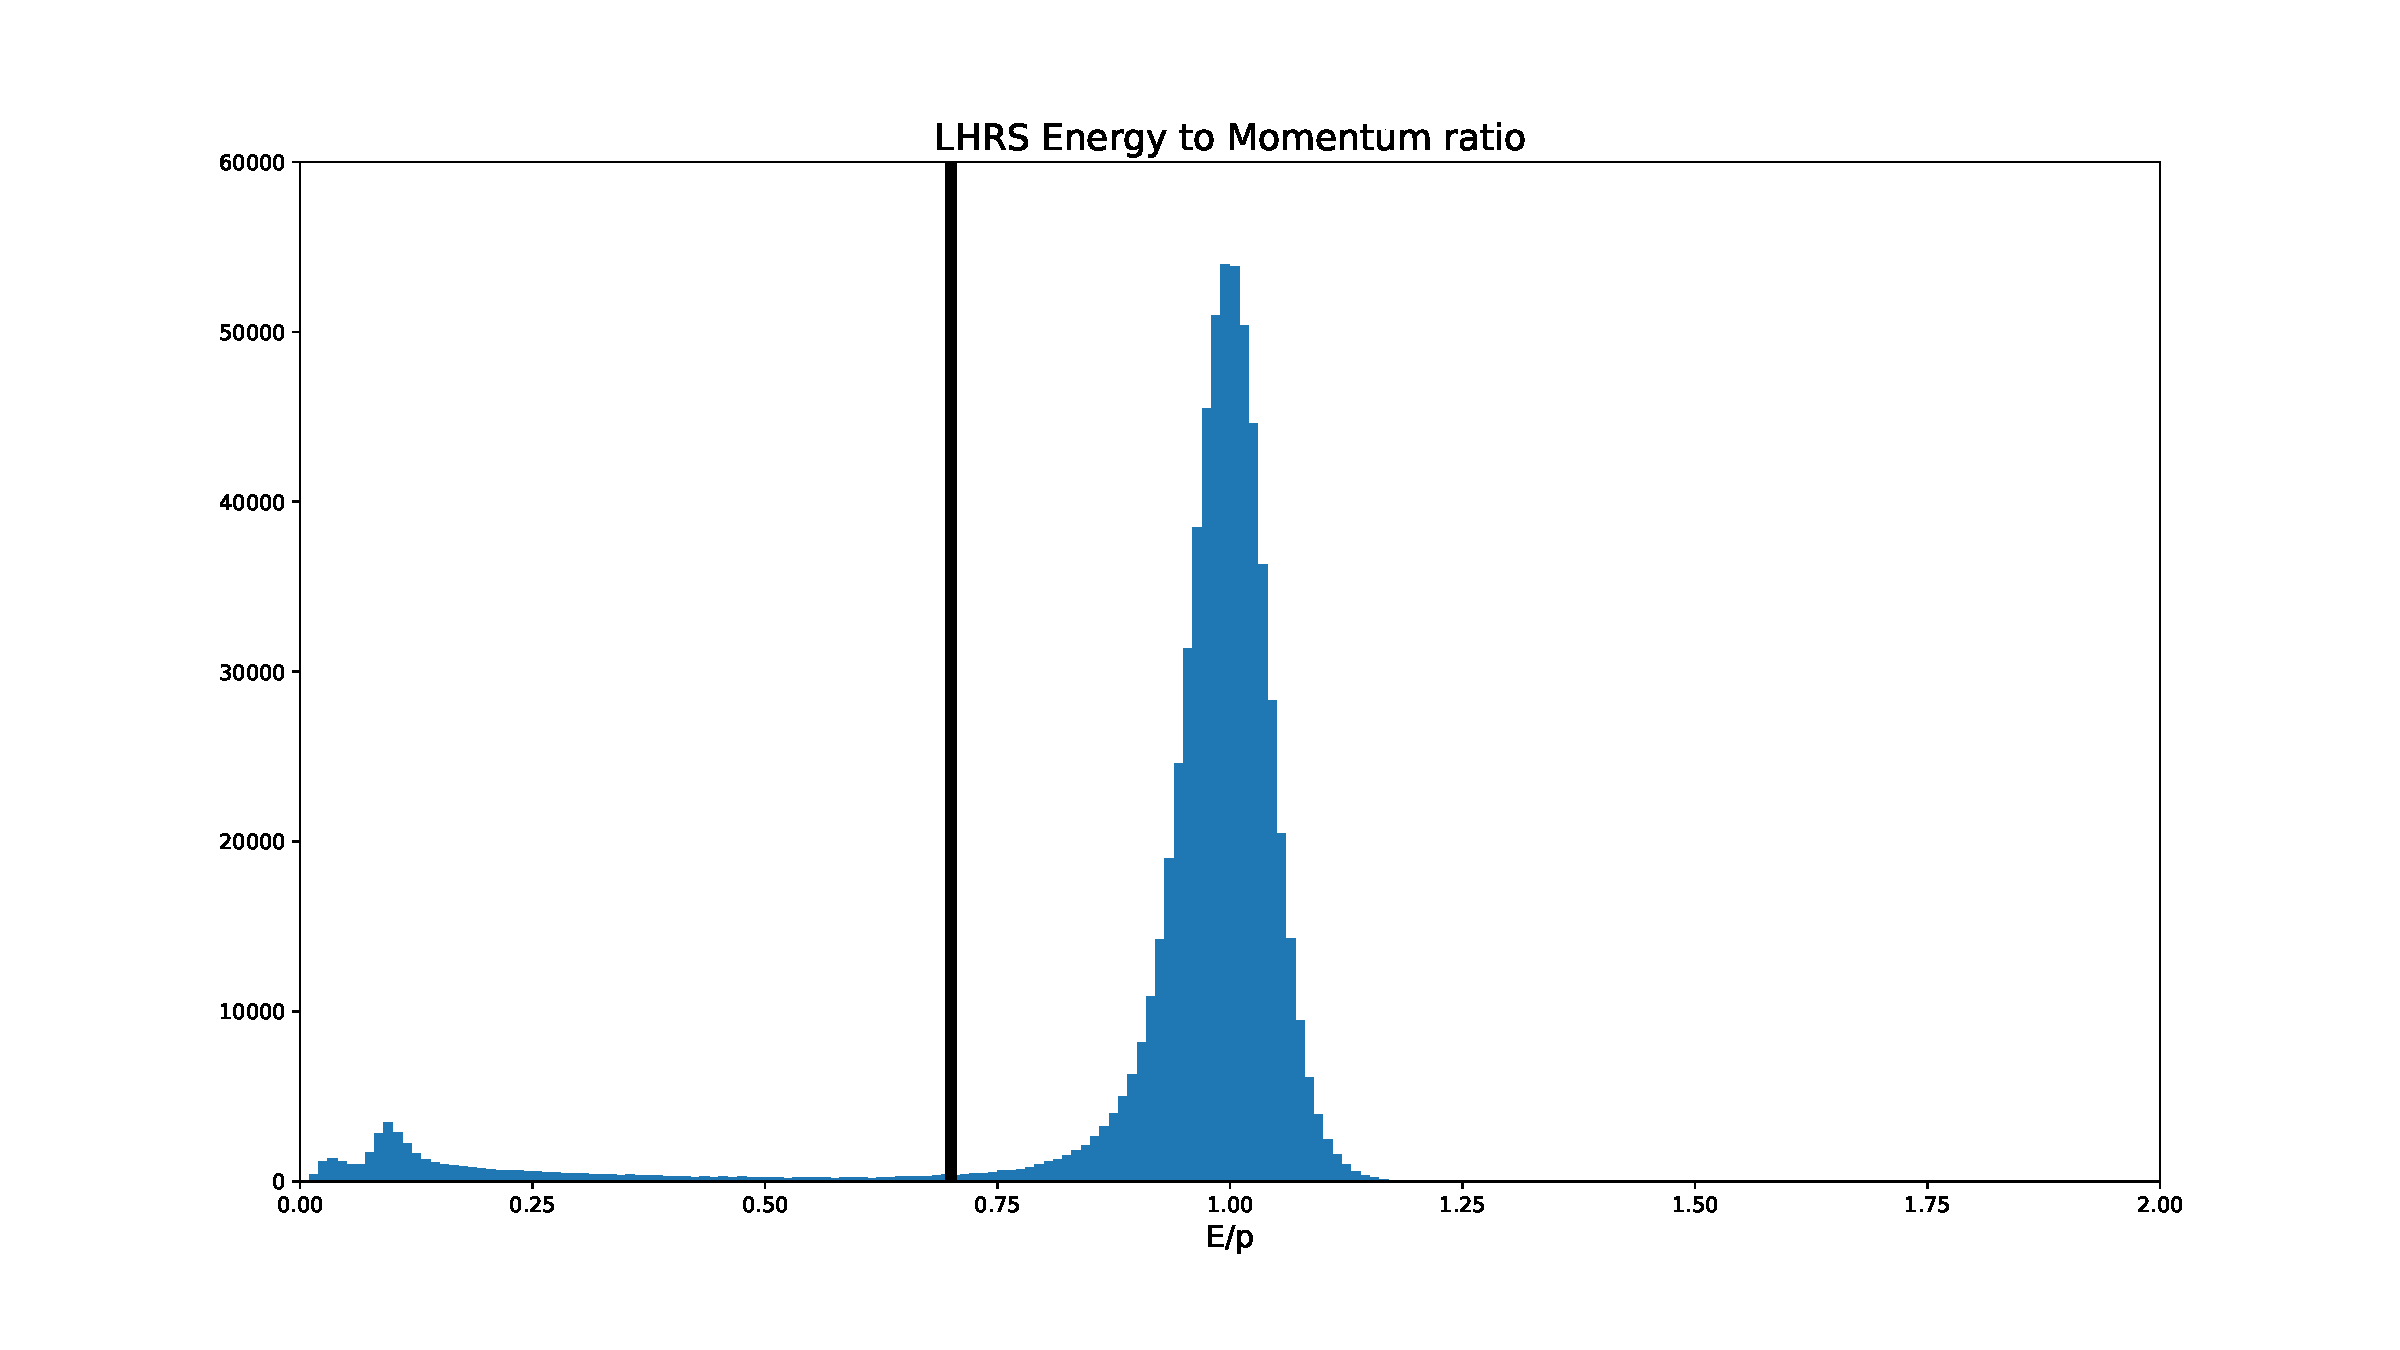
\includegraphics[width=\textwidth]{./analysis/fig/LCal_pid.pdf}
	\caption{This plot show the Calorimeter spectrum from the LHRS. All cuts are applied except for the PID cut on the Calorimeter. This plot shows events from kinematic 0. The black lines show the where the cuts are applied.}
	\label{fig:cal_pid}
\end{center}
\end{figure}

\begin{figure}
\begin{center}
	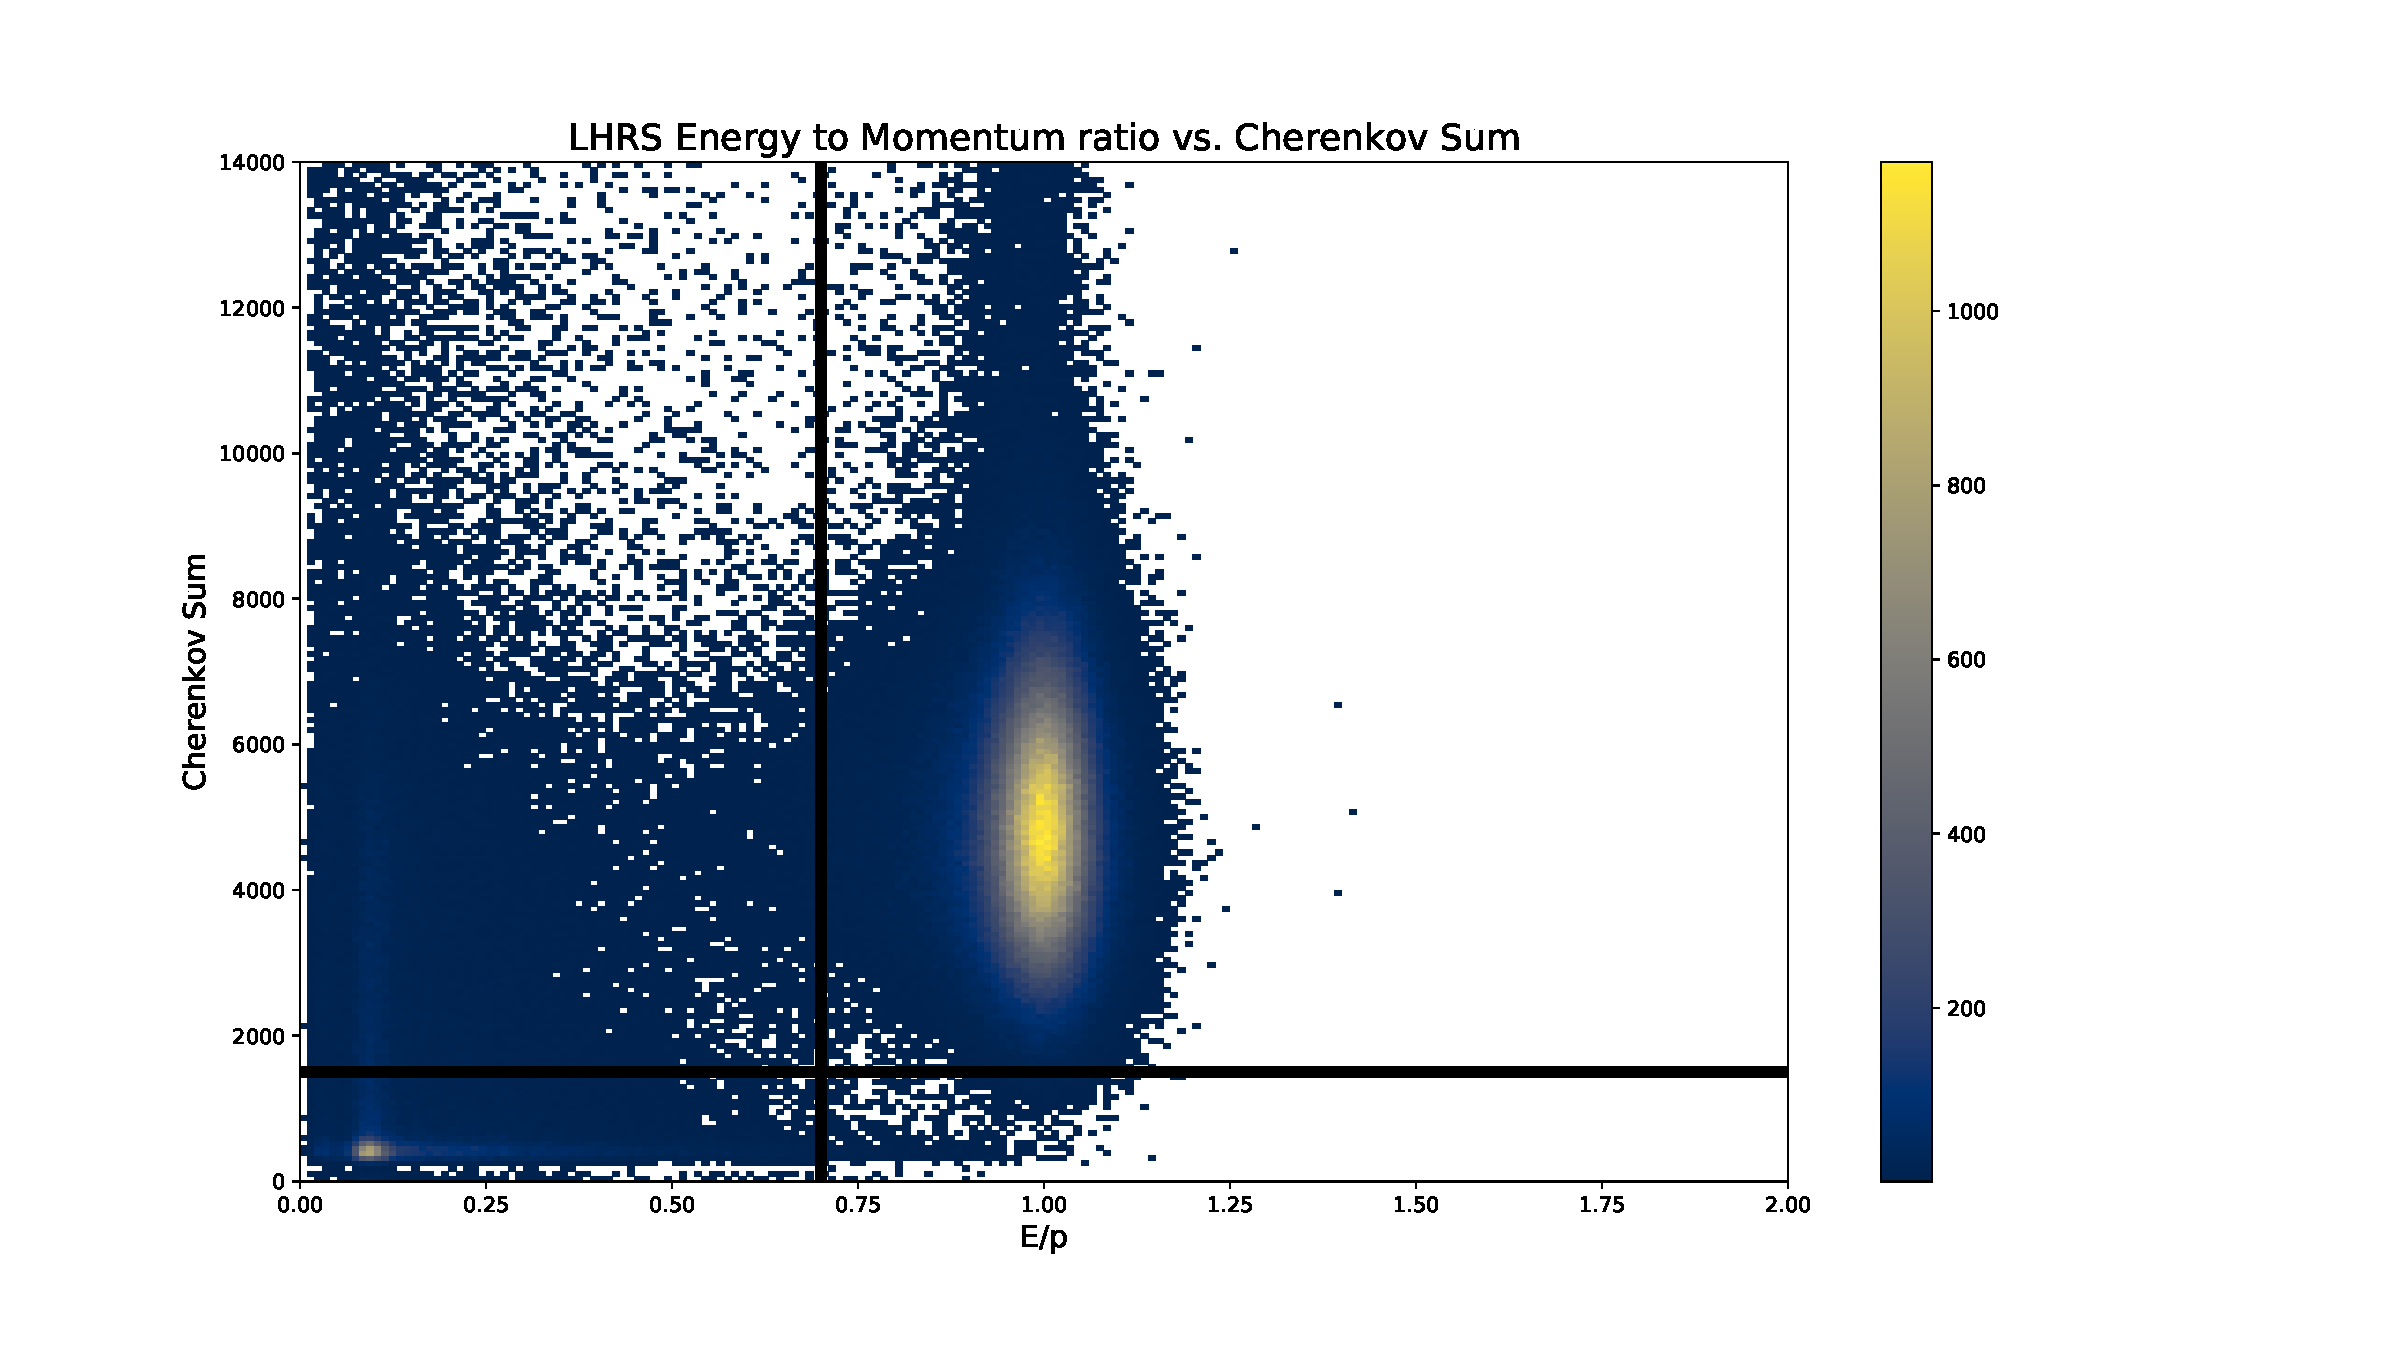
\includegraphics[width=\textwidth]{./analysis/fig/LCervCal_pid.pdf}
	\caption{This plot show the Calorimeter versus Cherenkov Sum spectra for the LHRS. All cuts are applied except for the PID cuts on the Cherenkov Sum and the Calorimeter. This plot shows events from kinematic 0. The black lines show the where the cuts are applied. The events in the upper-right corner pass the cuts and are considered to be good electrons.}
	\label{fig:cervcal_pid}
\end{center}
\end{figure}

\subsection{Acceptance}

Acceptance cuts are placed on the kinematic region that the spectrometer is sensitive to. These cuts are applied to the tracking variables ``Target $\phi$'', ``Target $\theta$'', and ``$\delta p$''. Target $\phi$ is a measure of the rotation in the plane of the hall floor. The value is the angular displacement from the central angle of the spectrometer. Target $\theta$ is the vertical angular displacement from the beam and target plane of the scattered electron. $\delta p$ is the deviation of the momentum of the scattered electron from the central momentum of the spectrometer. The RHRS also has a cut placed on the focal plane. These cuts are defined by examining the acceptance of the spectrometer. The cuts are placed around the area where the events are concentrated. The areas where events ``fell off'' were considered to be outside of the acceptance of the spectrometer. These cuts create a well defined acceptance band in the focal plane. In the RHRS, a very small number of events that passed these cuts were outside of this band. This led to a very loose cut being placed on the focal plane variables to omit these events. The acceptance regions for these variables are shown in Figures \ref{fig:acc} and \ref{fig:dp}. This is also how the focal plane cuts were determined for the RHRS, as shown in Figure \ref{fig:rfp}.

\begin{figure}
\begin{center}
	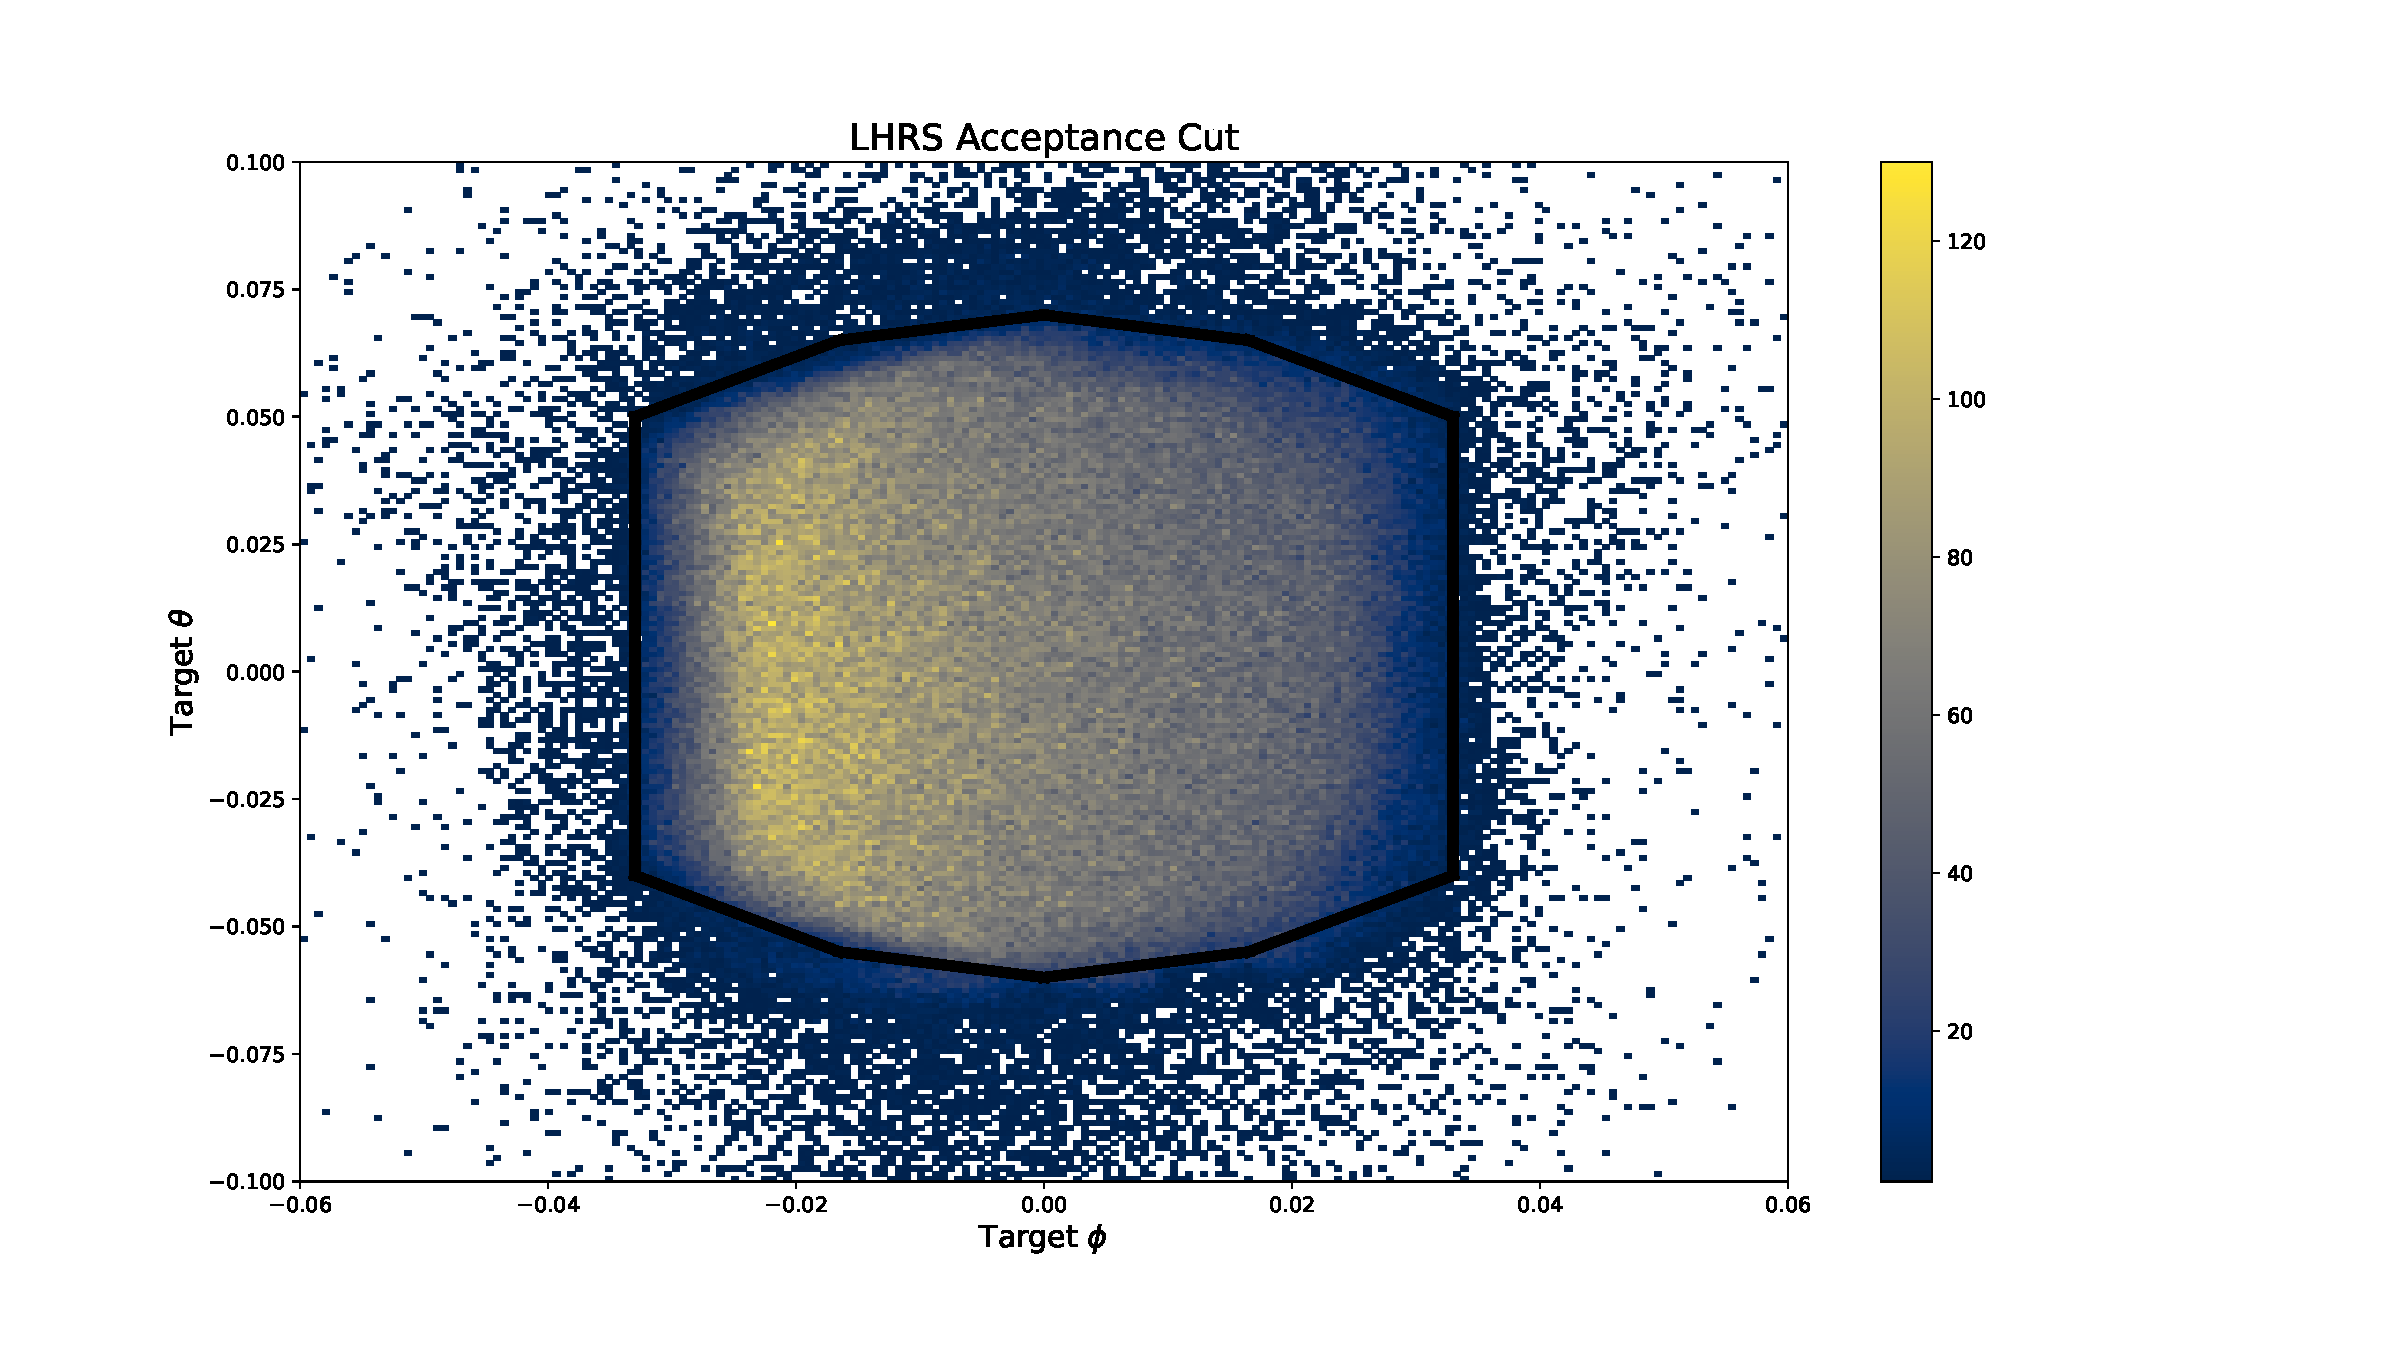
\includegraphics[width=\textwidth]{./analysis/fig/LHRS_ACC.pdf}
	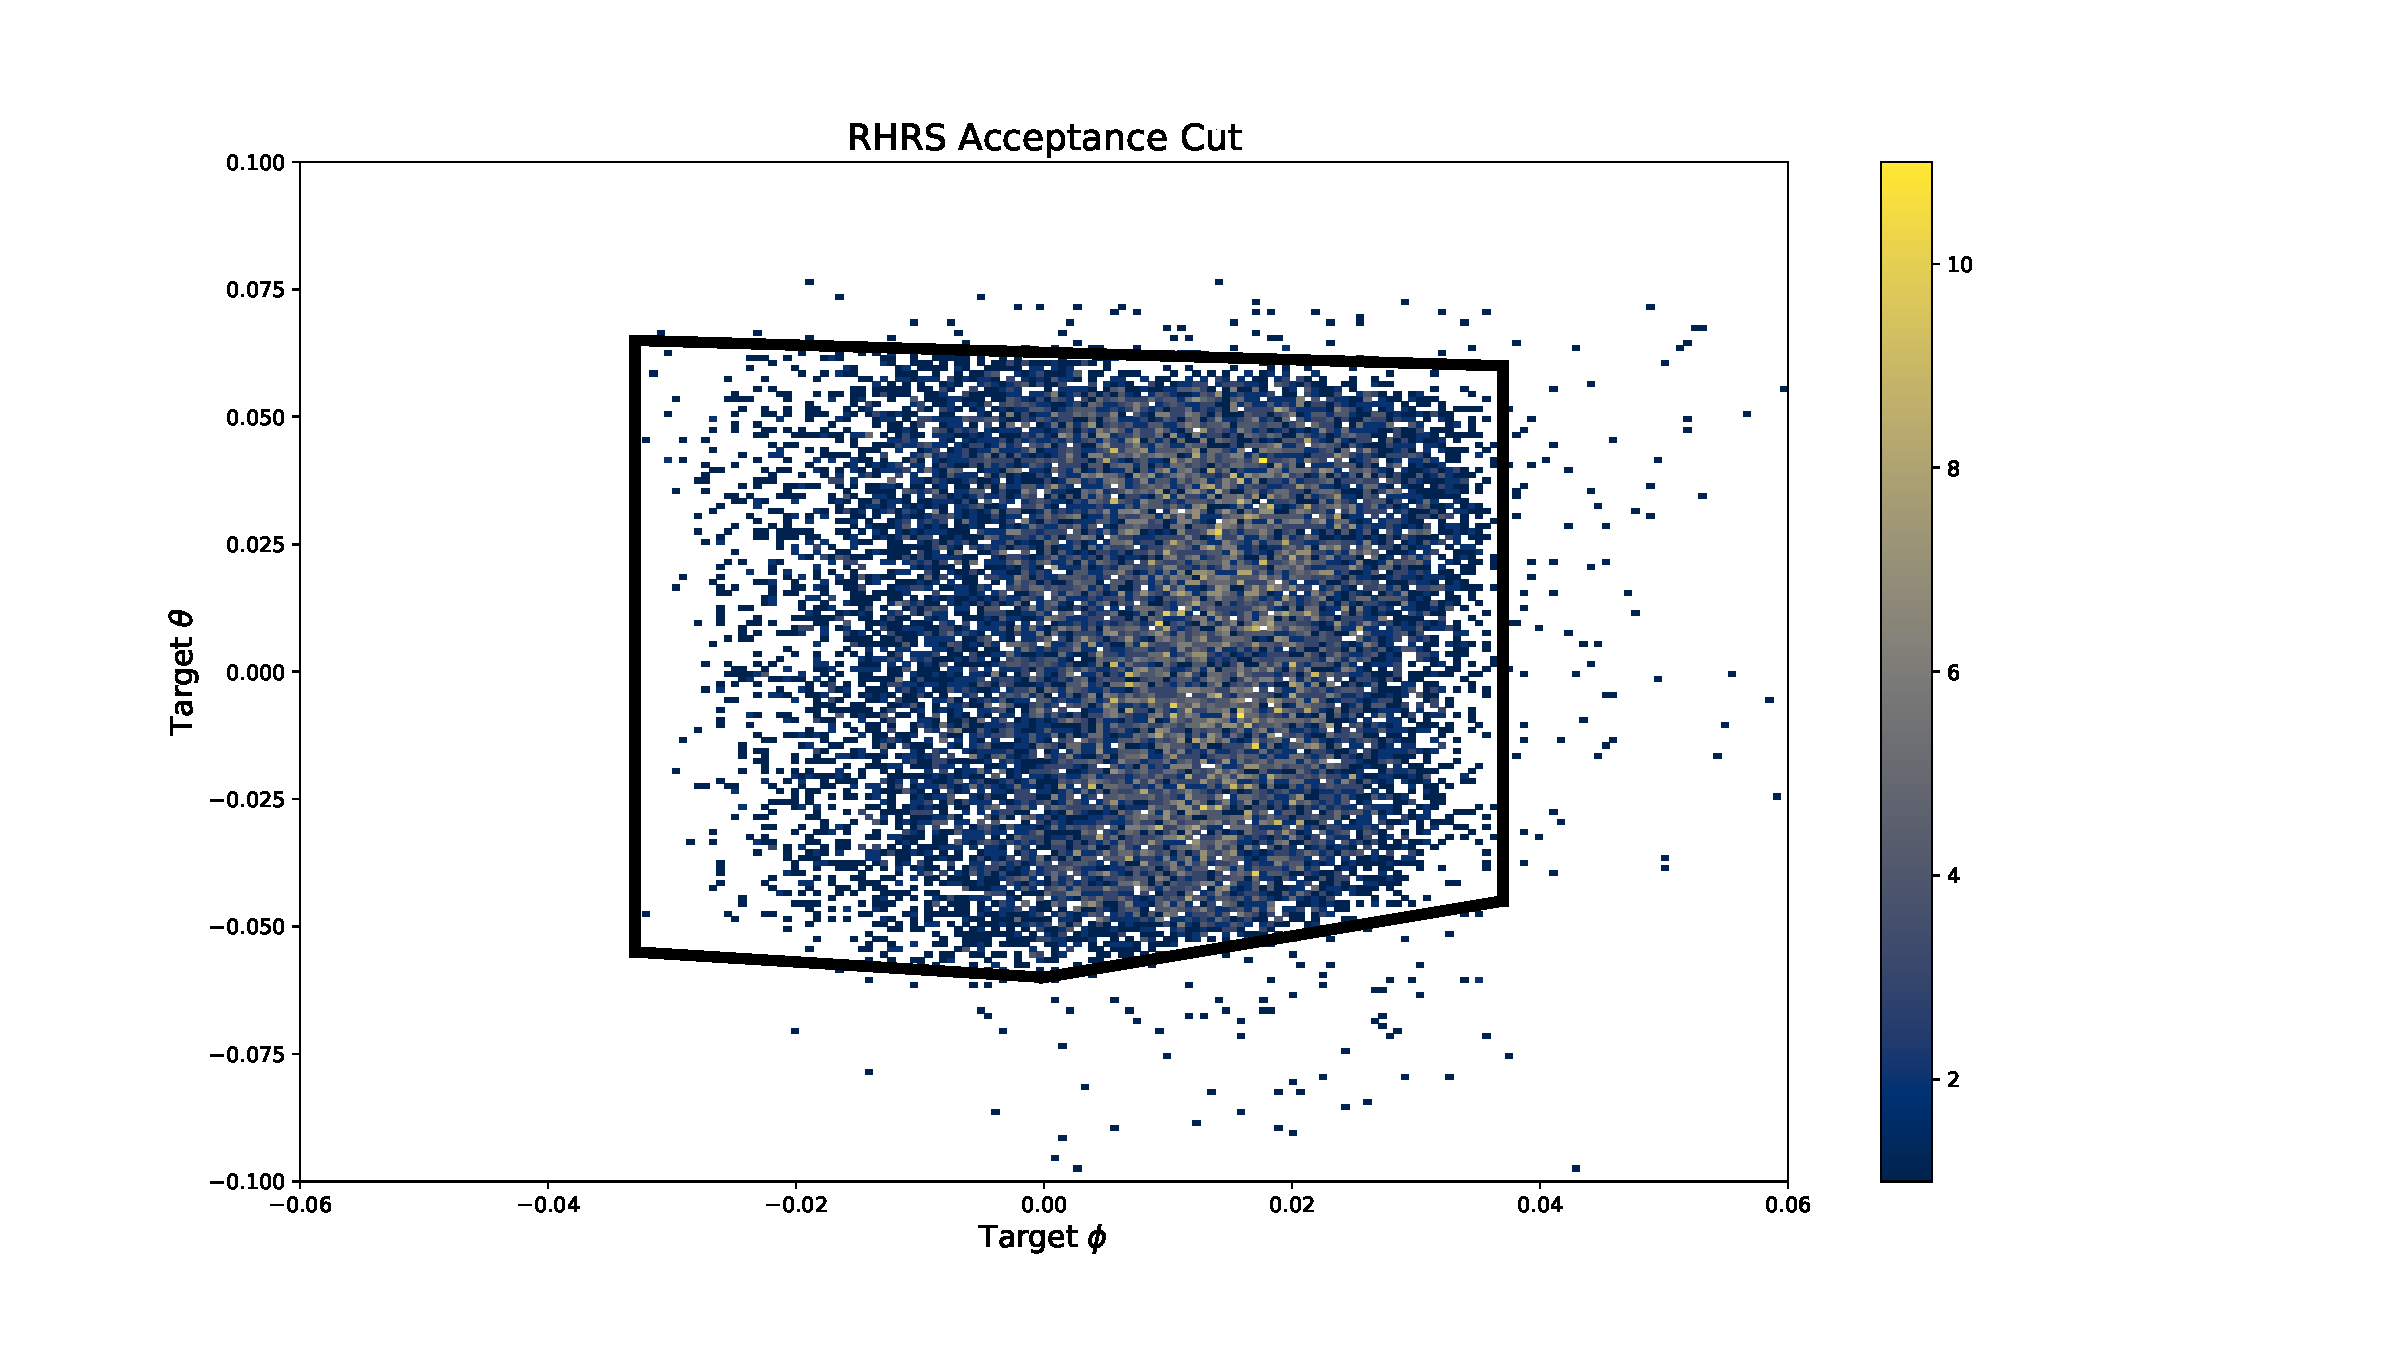
\includegraphics[width=\textwidth]{./analysis/fig/RHRS_ACC.pdf}
	\caption{These plots show the Target $\phi$ and Target $\theta$ acceptance variables of the spectrometer. All cuts are applied except for the Target $\phi$, Target $\theta$, and $\delta p$ cuts. The LHRS plot shows events from kinematic 0 while the RHRS plot shows events from kinematic 16. The black lines show the where the cuts are applied.}
	\label{fig:acc}
\end{center}
\end{figure}

\begin{figure}
\begin{center}
	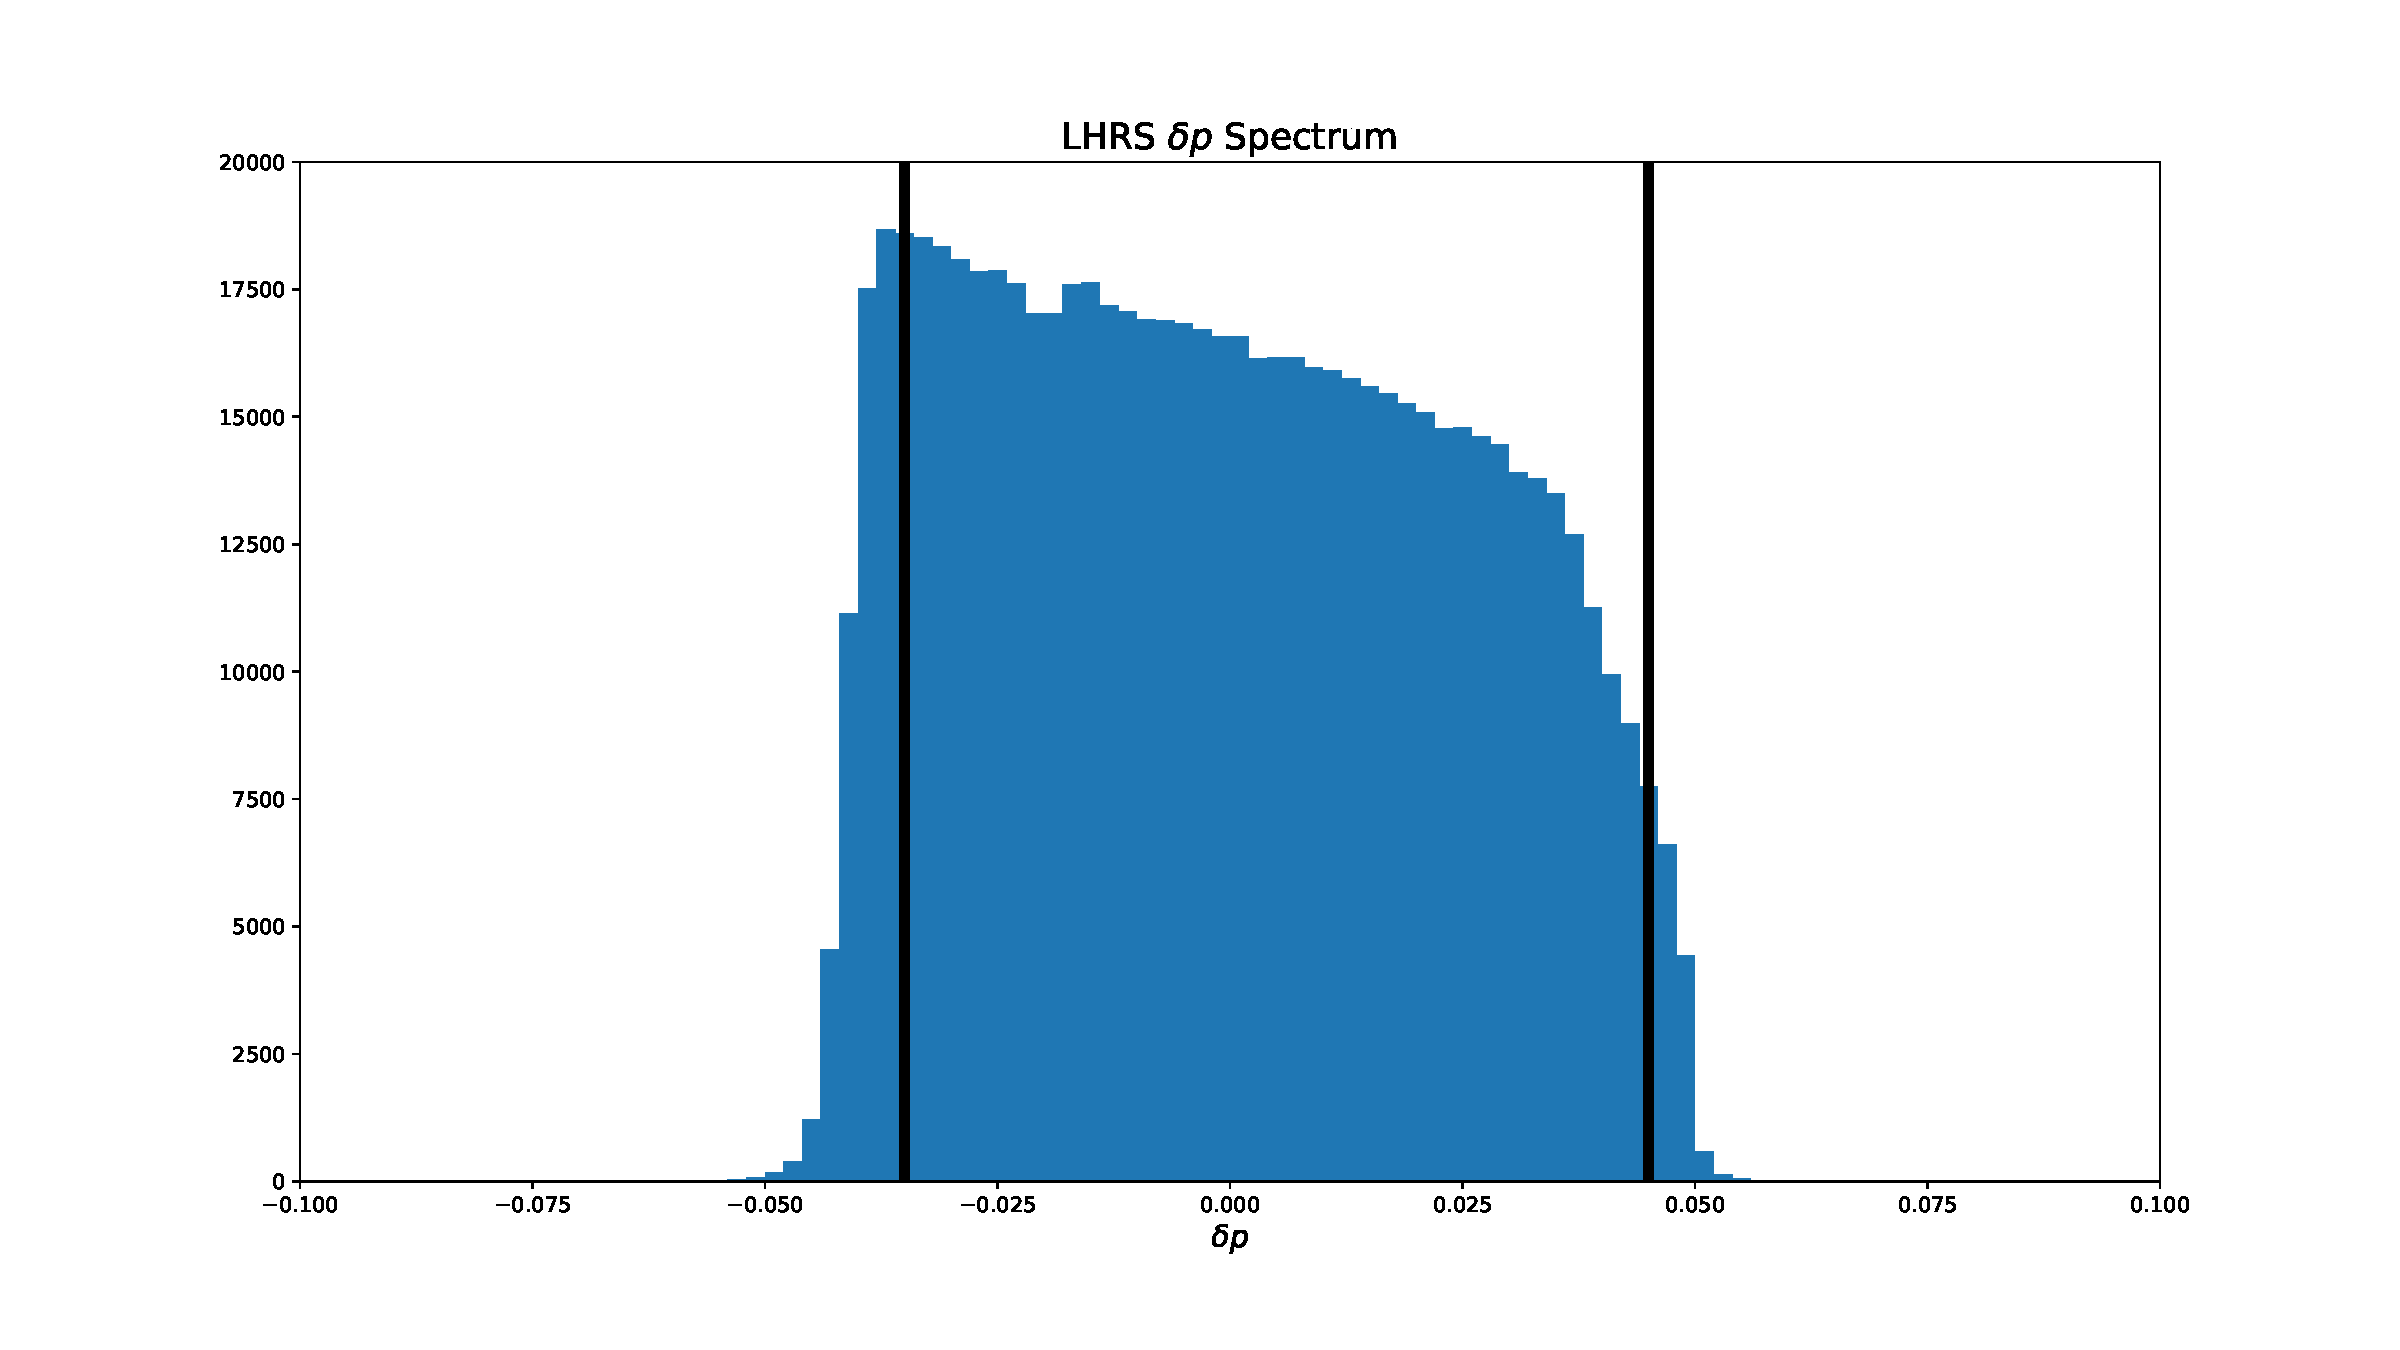
\includegraphics[width=\textwidth]{./analysis/fig/LHRS_dp.pdf}
	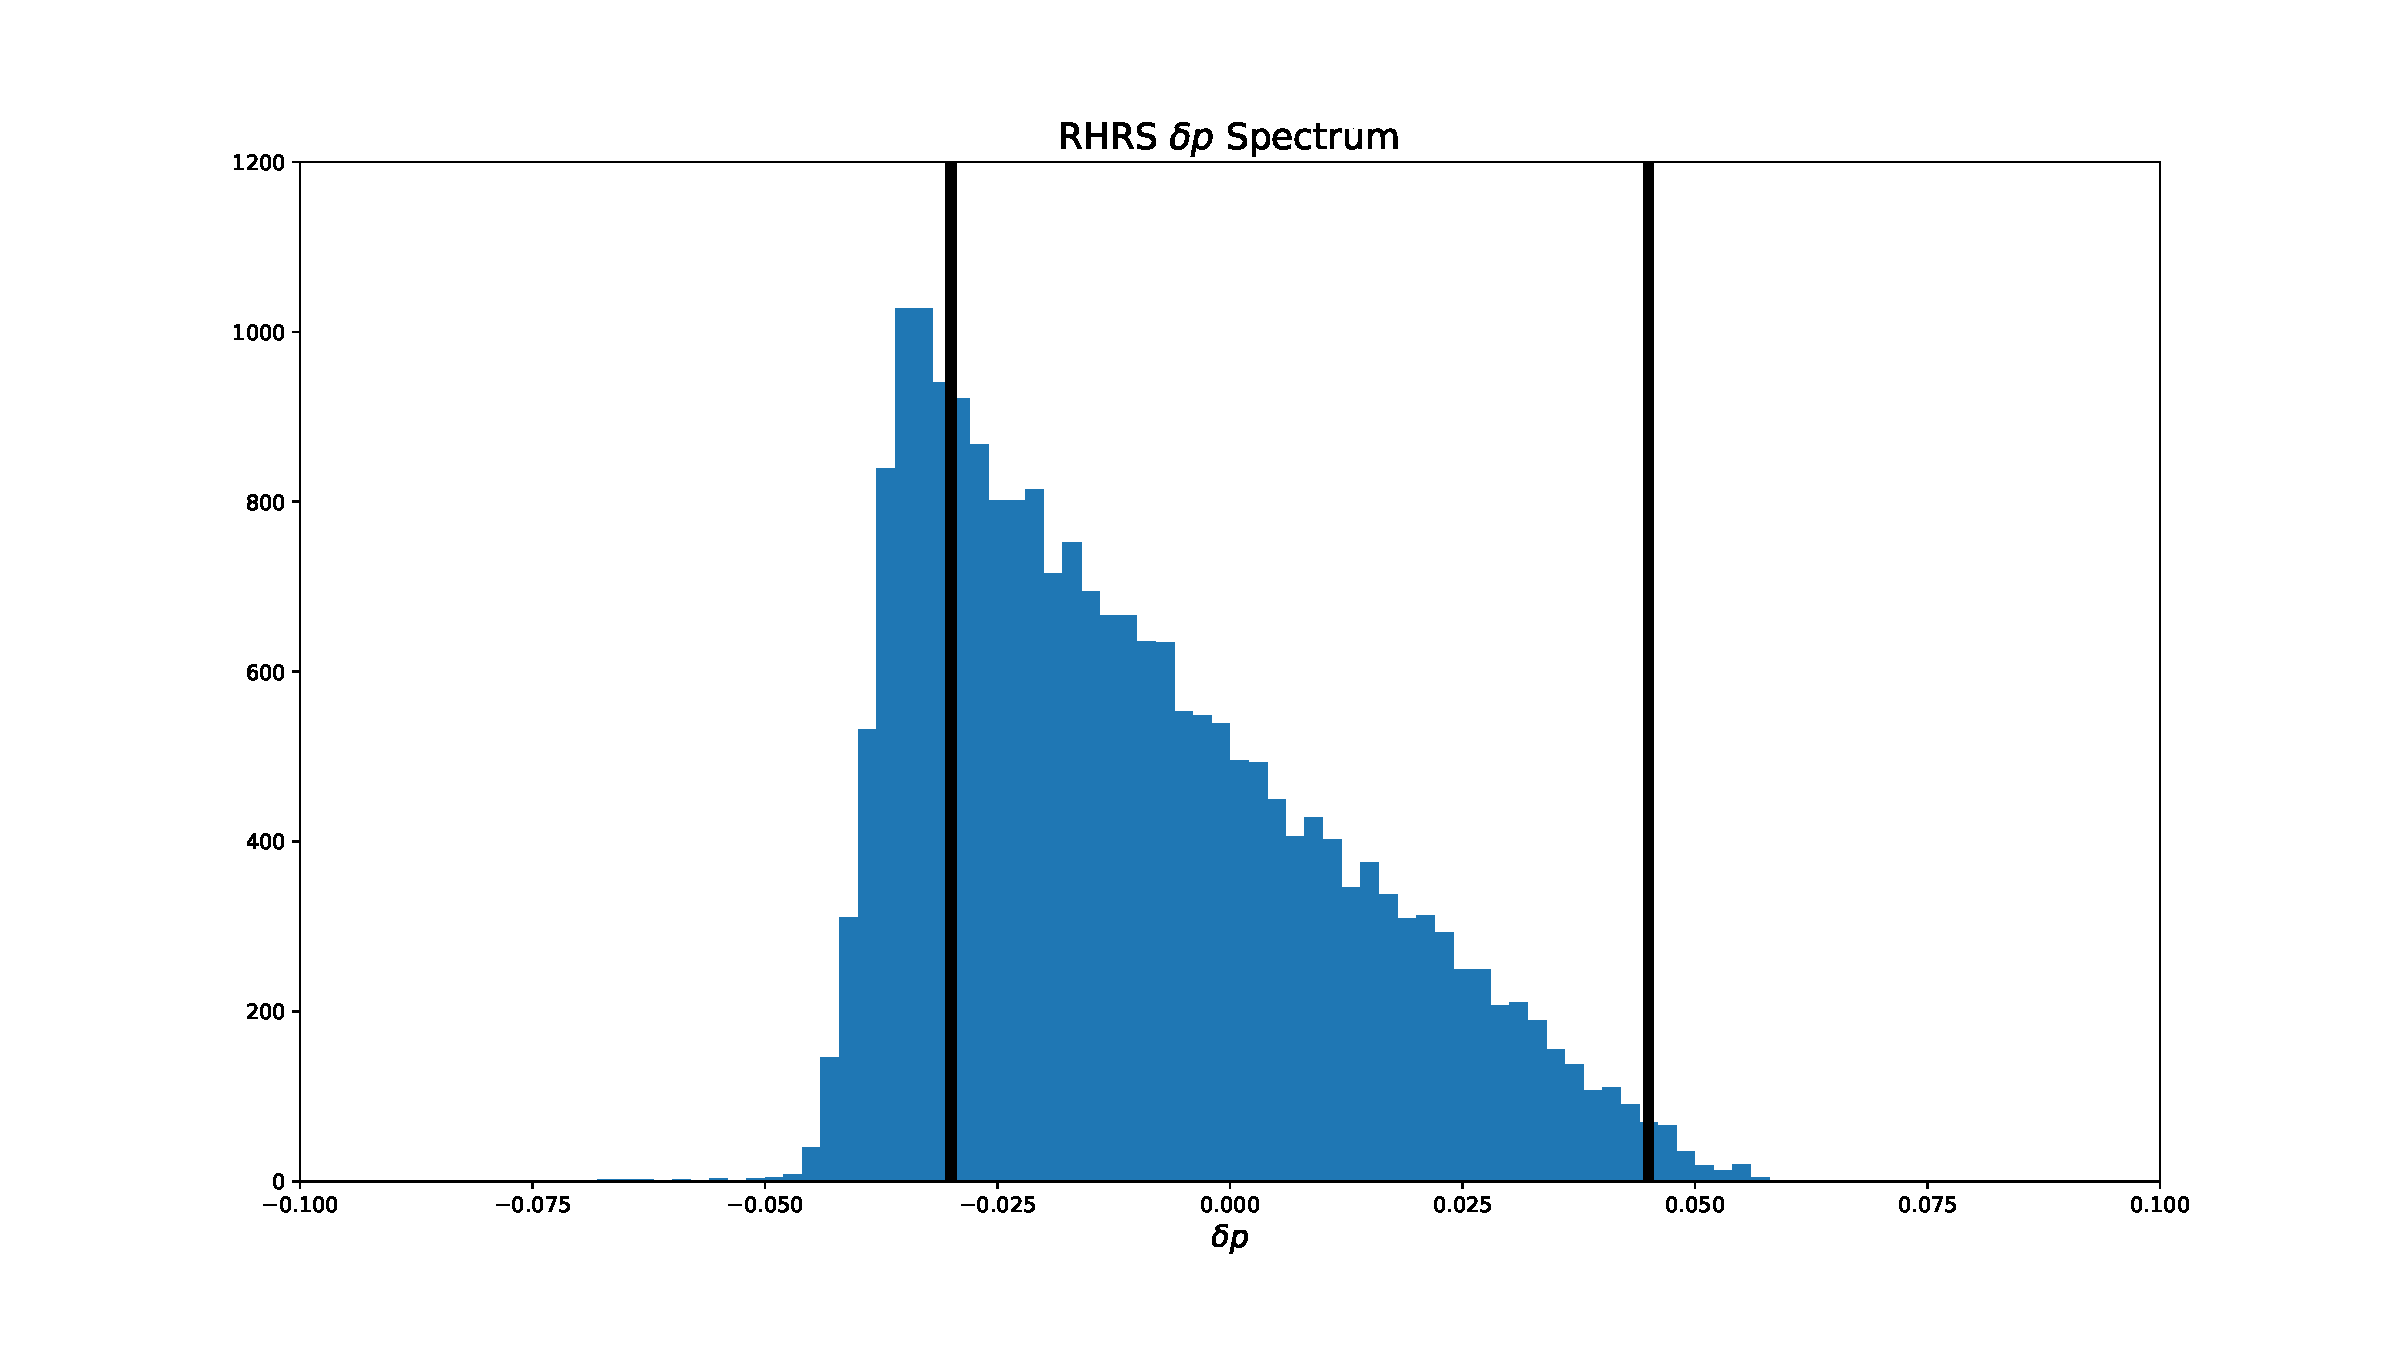
\includegraphics[width=\textwidth]{./analysis/fig/RHRS_dp.pdf}
	\caption{These plots show the $\delta p$ acceptance variable of the spectrometer. All cuts are applied except for the Target $\phi$, Target $\theta$, and $\delta p$ cuts. The LHRS plot shows events from kinematic 0 while the RHRS plot shows events from kinematic 16. The black lines show the where the cuts are applied.}
	\label{fig:dp}
\end{center}
\end{figure}

\begin{figure}
\begin{center}
	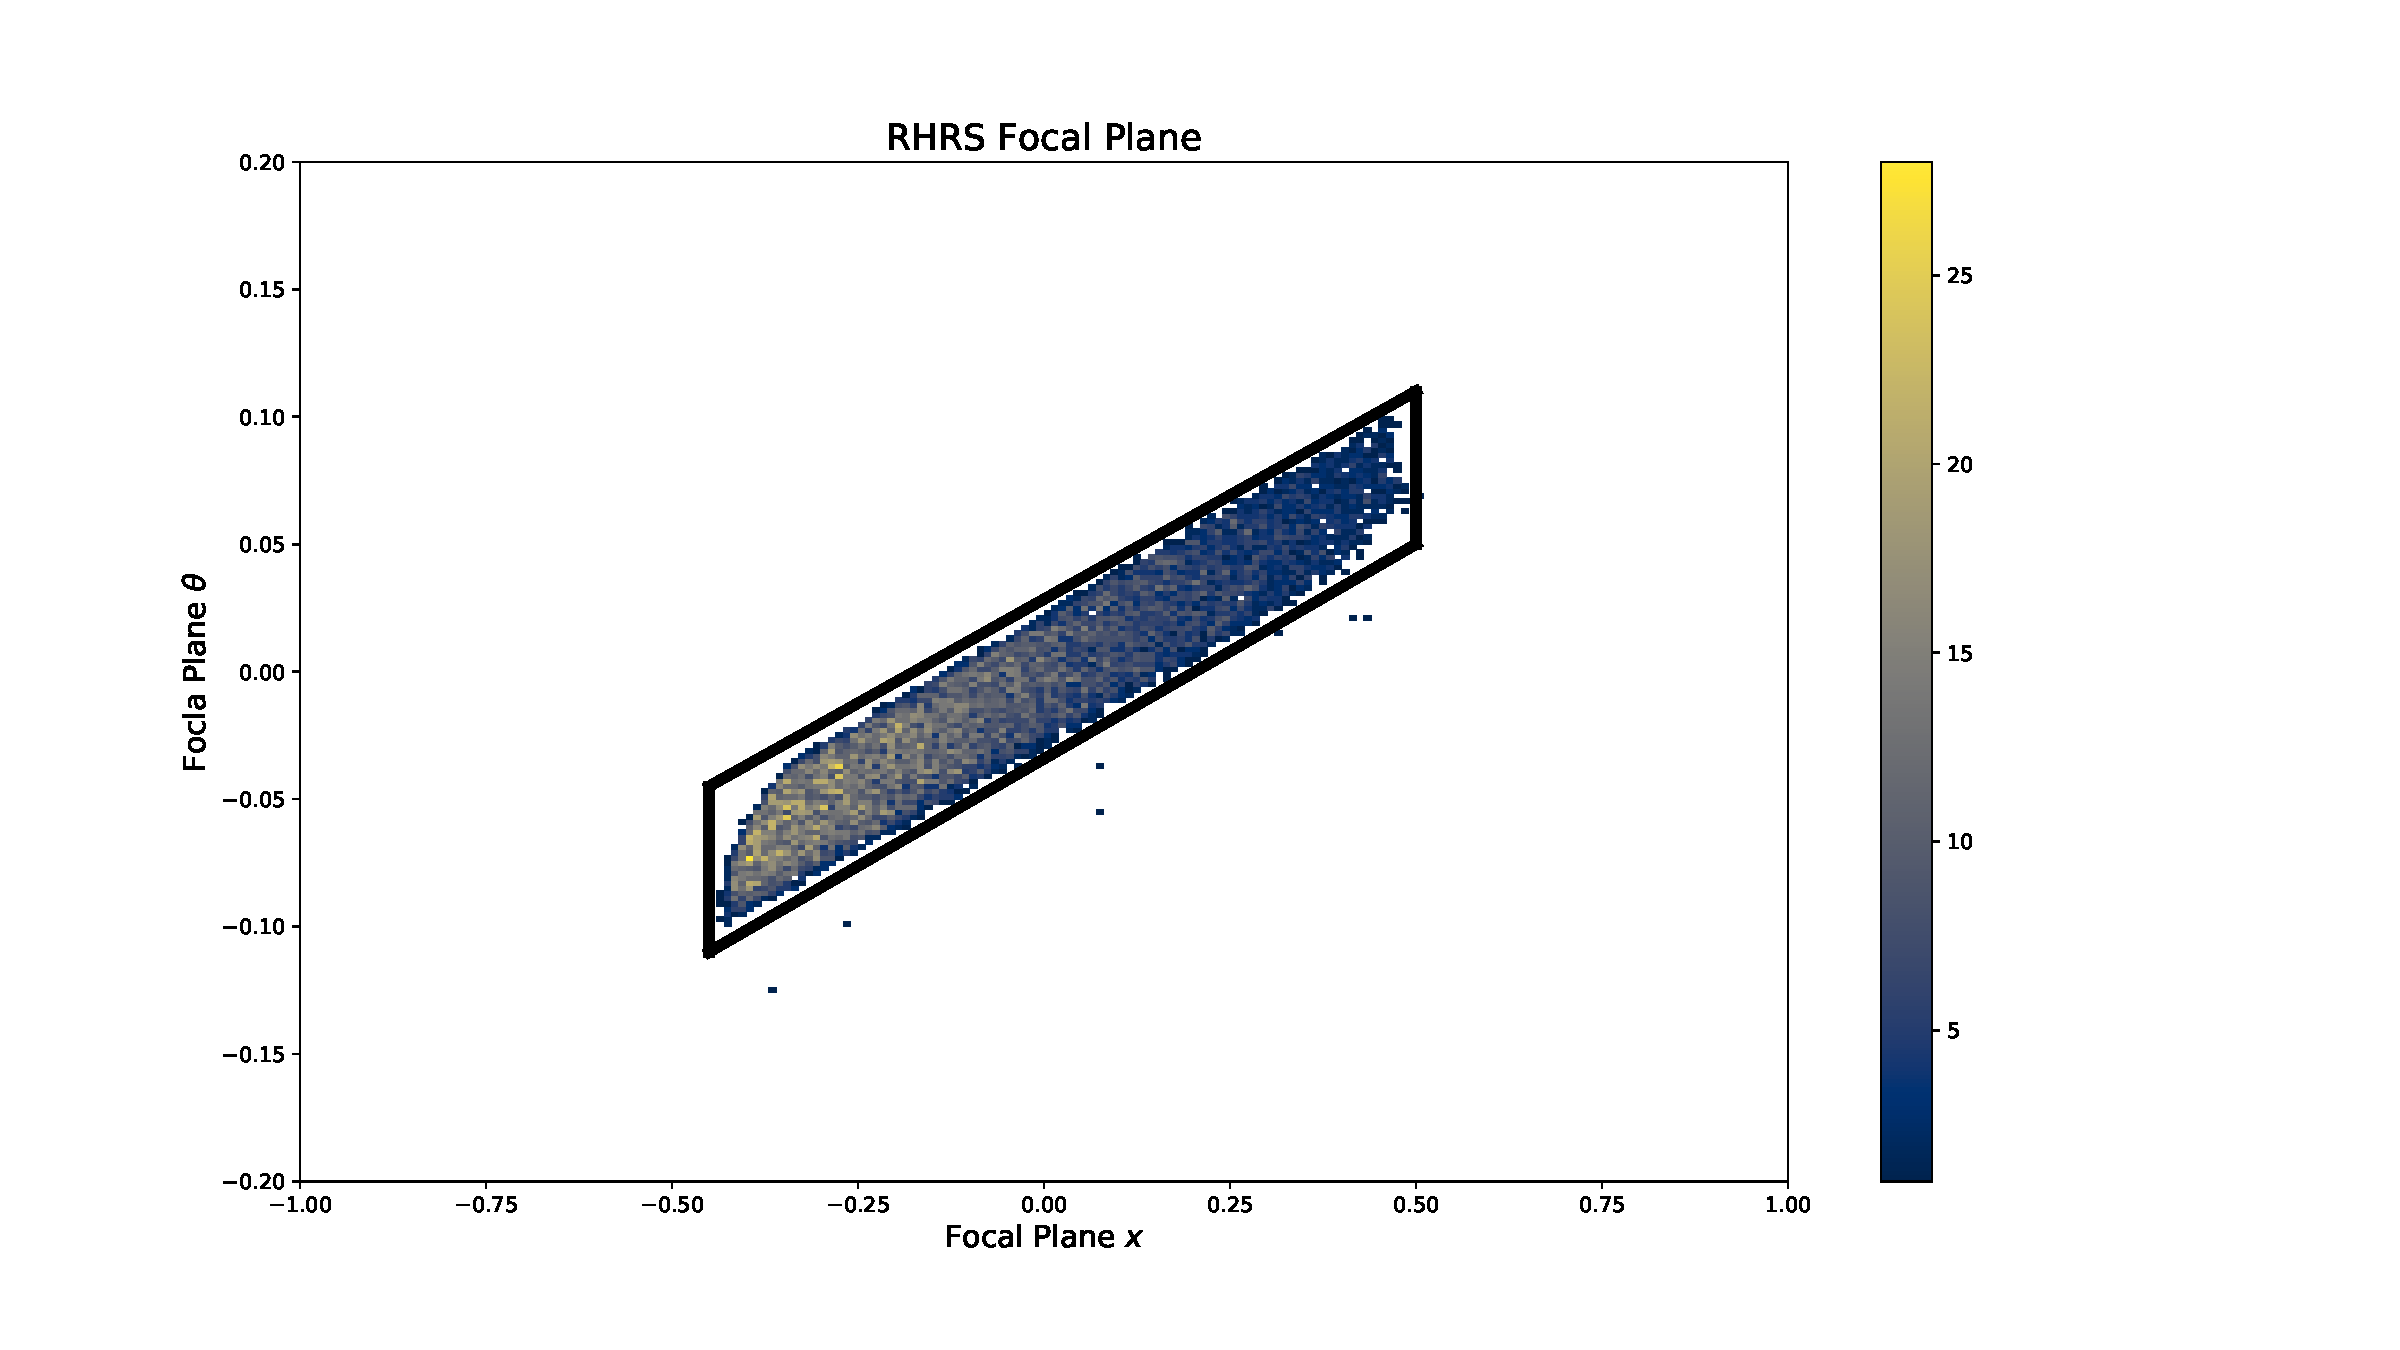
\includegraphics[width=\textwidth]{./analysis/fig/RHRS_fp.pdf}
	\caption{This plot shows the Focal Plane variables for RHRS kinematic 16. All cuts are applied. It was noted that after acceptance cuts were applied to RHRS data, there were still a few events that were not in the main region of the focal plane. A loose cut is applied to remove these events.}
	\label{fig:rfp}
\end{center}
\end{figure}

The other acceptance cut that is applied is to the target length. This cut is applied to the ``z-Target'' value of an event, where the event happened in the target along the axis of the beamline. This cut is used in order to minimize the amount of Endcap Contamination events that need to be corrected for. The cut is defined on a kinematic-by-kinematic basis, with higher kinematics having more of the target length allowed to pass the cut due to a smaller endcap contribution to the overall event rate. These cuts are defined in Table \ref{tbl:ztar}.

\begin{table}
\begin{center}
\begin{tabular}{|c|c|}
\hline
\textbf{Kinematics} & \textbf{z-Target Acceptance (m)}\\
\hline\hline
0 - 4 & $-0.08$ - $0.1$ \\ \hline
5 - 7 & $-0.09$ - $0.1$ \\ \hline
9 - 11 & $-0.095$ - $0.1$ \\ \hline
13 - 15 & $-0.1$ - $0.105$ \\ \hline
16 & $-0.105$ - $0.11$ \\ \hline
\end{tabular}
\caption{This table shows the range of the target, along the beam axis, that events are accepted from. This is done to minimize contamination from the endcaps of the targets.}
\label{tbl:ztar}
\end{center}
\end{table}